\documentclass[]{article}
\usepackage{lmodern}
\usepackage{amssymb,amsmath}
\usepackage{ifxetex,ifluatex}
\usepackage{fixltx2e} % provides \textsubscript
\ifnum 0\ifxetex 1\fi\ifluatex 1\fi=0 % if pdftex
  \usepackage[T1]{fontenc}
  \usepackage[utf8]{inputenc}
\else % if luatex or xelatex
  \ifxetex
    \usepackage{mathspec}
  \else
    \usepackage{fontspec}
  \fi
  \defaultfontfeatures{Ligatures=TeX,Scale=MatchLowercase}
\fi
% use upquote if available, for straight quotes in verbatim environments
\IfFileExists{upquote.sty}{\usepackage{upquote}}{}
% use microtype if available
\IfFileExists{microtype.sty}{%
\usepackage{microtype}
\UseMicrotypeSet[protrusion]{basicmath} % disable protrusion for tt fonts
}{}
\usepackage[margin=1in]{geometry}
\usepackage{hyperref}
\hypersetup{unicode=true,
            pdftitle={Scoring Evaluations},
            pdfauthor={Dave Bridges},
            pdfborder={0 0 0},
            breaklinks=true}
\urlstyle{same}  % don't use monospace font for urls
\usepackage{color}
\usepackage{fancyvrb}
\newcommand{\VerbBar}{|}
\newcommand{\VERB}{\Verb[commandchars=\\\{\}]}
\DefineVerbatimEnvironment{Highlighting}{Verbatim}{commandchars=\\\{\}}
% Add ',fontsize=\small' for more characters per line
\usepackage{framed}
\definecolor{shadecolor}{RGB}{248,248,248}
\newenvironment{Shaded}{\begin{snugshade}}{\end{snugshade}}
\newcommand{\KeywordTok}[1]{\textcolor[rgb]{0.13,0.29,0.53}{\textbf{{#1}}}}
\newcommand{\DataTypeTok}[1]{\textcolor[rgb]{0.13,0.29,0.53}{{#1}}}
\newcommand{\DecValTok}[1]{\textcolor[rgb]{0.00,0.00,0.81}{{#1}}}
\newcommand{\BaseNTok}[1]{\textcolor[rgb]{0.00,0.00,0.81}{{#1}}}
\newcommand{\FloatTok}[1]{\textcolor[rgb]{0.00,0.00,0.81}{{#1}}}
\newcommand{\ConstantTok}[1]{\textcolor[rgb]{0.00,0.00,0.00}{{#1}}}
\newcommand{\CharTok}[1]{\textcolor[rgb]{0.31,0.60,0.02}{{#1}}}
\newcommand{\SpecialCharTok}[1]{\textcolor[rgb]{0.00,0.00,0.00}{{#1}}}
\newcommand{\StringTok}[1]{\textcolor[rgb]{0.31,0.60,0.02}{{#1}}}
\newcommand{\VerbatimStringTok}[1]{\textcolor[rgb]{0.31,0.60,0.02}{{#1}}}
\newcommand{\SpecialStringTok}[1]{\textcolor[rgb]{0.31,0.60,0.02}{{#1}}}
\newcommand{\ImportTok}[1]{{#1}}
\newcommand{\CommentTok}[1]{\textcolor[rgb]{0.56,0.35,0.01}{\textit{{#1}}}}
\newcommand{\DocumentationTok}[1]{\textcolor[rgb]{0.56,0.35,0.01}{\textbf{\textit{{#1}}}}}
\newcommand{\AnnotationTok}[1]{\textcolor[rgb]{0.56,0.35,0.01}{\textbf{\textit{{#1}}}}}
\newcommand{\CommentVarTok}[1]{\textcolor[rgb]{0.56,0.35,0.01}{\textbf{\textit{{#1}}}}}
\newcommand{\OtherTok}[1]{\textcolor[rgb]{0.56,0.35,0.01}{{#1}}}
\newcommand{\FunctionTok}[1]{\textcolor[rgb]{0.00,0.00,0.00}{{#1}}}
\newcommand{\VariableTok}[1]{\textcolor[rgb]{0.00,0.00,0.00}{{#1}}}
\newcommand{\ControlFlowTok}[1]{\textcolor[rgb]{0.13,0.29,0.53}{\textbf{{#1}}}}
\newcommand{\OperatorTok}[1]{\textcolor[rgb]{0.81,0.36,0.00}{\textbf{{#1}}}}
\newcommand{\BuiltInTok}[1]{{#1}}
\newcommand{\ExtensionTok}[1]{{#1}}
\newcommand{\PreprocessorTok}[1]{\textcolor[rgb]{0.56,0.35,0.01}{\textit{{#1}}}}
\newcommand{\AttributeTok}[1]{\textcolor[rgb]{0.77,0.63,0.00}{{#1}}}
\newcommand{\RegionMarkerTok}[1]{{#1}}
\newcommand{\InformationTok}[1]{\textcolor[rgb]{0.56,0.35,0.01}{\textbf{\textit{{#1}}}}}
\newcommand{\WarningTok}[1]{\textcolor[rgb]{0.56,0.35,0.01}{\textbf{\textit{{#1}}}}}
\newcommand{\AlertTok}[1]{\textcolor[rgb]{0.94,0.16,0.16}{{#1}}}
\newcommand{\ErrorTok}[1]{\textcolor[rgb]{0.64,0.00,0.00}{\textbf{{#1}}}}
\newcommand{\NormalTok}[1]{{#1}}
\usepackage{graphicx,grffile}
\makeatletter
\def\maxwidth{\ifdim\Gin@nat@width>\linewidth\linewidth\else\Gin@nat@width\fi}
\def\maxheight{\ifdim\Gin@nat@height>\textheight\textheight\else\Gin@nat@height\fi}
\makeatother
% Scale images if necessary, so that they will not overflow the page
% margins by default, and it is still possible to overwrite the defaults
% using explicit options in \includegraphics[width, height, ...]{}
\setkeys{Gin}{width=\maxwidth,height=\maxheight,keepaspectratio}
\IfFileExists{parskip.sty}{%
\usepackage{parskip}
}{% else
\setlength{\parindent}{0pt}
\setlength{\parskip}{6pt plus 2pt minus 1pt}
}
\setlength{\emergencystretch}{3em}  % prevent overfull lines
\providecommand{\tightlist}{%
  \setlength{\itemsep}{0pt}\setlength{\parskip}{0pt}}
\setcounter{secnumdepth}{0}
% Redefines (sub)paragraphs to behave more like sections
\ifx\paragraph\undefined\else
\let\oldparagraph\paragraph
\renewcommand{\paragraph}[1]{\oldparagraph{#1}\mbox{}}
\fi
\ifx\subparagraph\undefined\else
\let\oldsubparagraph\subparagraph
\renewcommand{\subparagraph}[1]{\oldsubparagraph{#1}\mbox{}}
\fi

%%% Use protect on footnotes to avoid problems with footnotes in titles
\let\rmarkdownfootnote\footnote%
\def\footnote{\protect\rmarkdownfootnote}

%%% Change title format to be more compact
\usepackage{titling}

% Create subtitle command for use in maketitle
\newcommand{\subtitle}[1]{
  \posttitle{
    \begin{center}\large#1\end{center}
    }
}

\setlength{\droptitle}{-2em}
  \title{Scoring Evaluations}
  \pretitle{\vspace{\droptitle}\centering\huge}
  \posttitle{\par}
  \author{Dave Bridges}
  \preauthor{\centering\large\emph}
  \postauthor{\par}
  \predate{\centering\large\emph}
  \postdate{\par}
  \date{1/31/2018}


\begin{document}
\maketitle

{
\setcounter{tocdepth}{2}
\tableofcontents
}
\subsection{Data Import}\label{data-import}

Exported \textbf{Assignment Type Summaries} from GradeCraft and
imported.

\begin{Shaded}
\begin{Highlighting}[]
\KeywordTok{library}\NormalTok{(readr)}
\KeywordTok{library}\NormalTok{(dplyr)}
\KeywordTok{library}\NormalTok{(tidyr)}
\NormalTok{datafile <-}\StringTok{ 'Principles of Nutritional Sciences Assignment Type Summary - 2018-02-01.csv'}

\KeywordTok{library}\NormalTok{(readr)}
\NormalTok{dataset <-}\StringTok{ }\KeywordTok{read_csv}\NormalTok{(datafile)}

\NormalTok{dropped.students <-}\StringTok{ }\KeywordTok{c}\NormalTok{(}\StringTok{'dave.bridges'}\NormalTok{,}\StringTok{'ajian'}\NormalTok{,}\StringTok{'zhongyli'}\NormalTok{)}

\NormalTok{assessment.dataset <-}
\StringTok{  }\NormalTok{dataset %>%}
\StringTok{  }\KeywordTok{select}\NormalTok{(-}\StringTok{`}\DataTypeTok{First Name}\StringTok{`}\NormalTok{, -}\StringTok{`}\DataTypeTok{Last Name}\StringTok{`}\NormalTok{, -Email, -Team) %>%}
\StringTok{  }\KeywordTok{gather}\NormalTok{(Assignment, Points, -Username) %>%}\StringTok{ }
\StringTok{  }\KeywordTok{filter}\NormalTok{(!(Username %in%}\StringTok{ }\NormalTok{dropped.students)) %>%}
\StringTok{  }\KeywordTok{arrange}\NormalTok{(Points)}

\NormalTok{summary.dataset <-}
\StringTok{  }\NormalTok{assessment.dataset %>%}
\StringTok{  }\KeywordTok{group_by}\NormalTok{(Username) %>%}
\StringTok{  }\KeywordTok{summarize}\NormalTok{(}\DataTypeTok{Total =} \KeywordTok{sum}\NormalTok{(Points)) %>%}
\StringTok{  }\KeywordTok{arrange}\NormalTok{(-Total)}
\end{Highlighting}
\end{Shaded}

This script imports the data from \textbf{Principles of Nutritional
Sciences Assignment Type Summary - 2018-02-01.csv}. This script is
located at
/Users/davebrid/Documents/GitHub/TeachingLectures/Michigan/NUTR630/Evaluation/GradeCraft
Summary/GradeCraft Metrics and was most recently run on Wed Jan 31
21:50:10 2018

\begin{Shaded}
\begin{Highlighting}[]
\KeywordTok{library}\NormalTok{(ggplot2)}

\NormalTok{p <-}\StringTok{ }\KeywordTok{ggplot}\NormalTok{(}\DataTypeTok{data=}\NormalTok{summary.dataset, }\KeywordTok{aes}\NormalTok{(}\DataTypeTok{x=}\NormalTok{Total)) }
\NormalTok{p +}\StringTok{ }\KeywordTok{geom_histogram}\NormalTok{(}\DataTypeTok{binwidth=}\DecValTok{50}\NormalTok{) +}
\StringTok{  }\KeywordTok{labs}\NormalTok{(}\DataTypeTok{x=}\StringTok{"Final Points"}\NormalTok{,}\DataTypeTok{y=}\StringTok{"Number of Students"}\NormalTok{, }\DataTypeTok{title=}\StringTok{"Distribution of Final Points"}\NormalTok{) +}
\StringTok{  }\KeywordTok{geom_vline}\NormalTok{(}\KeywordTok{aes}\NormalTok{(}\DataTypeTok{xintercept=}\DecValTok{1000}\NormalTok{), }\DataTypeTok{color=}\StringTok{"red"}\NormalTok{, }\DataTypeTok{linetype=}\StringTok{"dashed"}\NormalTok{, }\DataTypeTok{size=}\DecValTok{1}\NormalTok{) +}
\StringTok{  }\KeywordTok{geom_vline}\NormalTok{(}\KeywordTok{aes}\NormalTok{(}\DataTypeTok{xintercept=}\DecValTok{950}\NormalTok{), }\DataTypeTok{color=}\StringTok{"red"}\NormalTok{, }\DataTypeTok{linetype=}\StringTok{"dashed"}\NormalTok{, }\DataTypeTok{size=}\FloatTok{0.5}\NormalTok{) +}
\StringTok{  }\KeywordTok{geom_vline}\NormalTok{(}\KeywordTok{aes}\NormalTok{(}\DataTypeTok{xintercept=}\DecValTok{900}\NormalTok{), }\DataTypeTok{color=}\StringTok{"red"}\NormalTok{, }\DataTypeTok{linetype=}\StringTok{"dashed"}\NormalTok{, }\DataTypeTok{size=}\FloatTok{0.5}\NormalTok{) +}
\StringTok{  }\KeywordTok{geom_vline}\NormalTok{(}\KeywordTok{aes}\NormalTok{(}\DataTypeTok{xintercept=}\DecValTok{850}\NormalTok{), }\DataTypeTok{color=}\StringTok{"red"}\NormalTok{, }\DataTypeTok{linetype=}\StringTok{"dashed"}\NormalTok{, }\DataTypeTok{size=}\FloatTok{0.5}\NormalTok{) +}
\StringTok{  }\KeywordTok{geom_vline}\NormalTok{(}\KeywordTok{aes}\NormalTok{(}\DataTypeTok{xintercept=}\DecValTok{800}\NormalTok{), }\DataTypeTok{color=}\StringTok{"red"}\NormalTok{, }\DataTypeTok{linetype=}\StringTok{"dashed"}\NormalTok{, }\DataTypeTok{size=}\FloatTok{0.5}\NormalTok{) +}
\StringTok{  }\KeywordTok{geom_vline}\NormalTok{(}\KeywordTok{aes}\NormalTok{(}\DataTypeTok{xintercept=}\DecValTok{750}\NormalTok{), }\DataTypeTok{color=}\StringTok{"red"}\NormalTok{, }\DataTypeTok{linetype=}\StringTok{"dashed"}\NormalTok{, }\DataTypeTok{size=}\FloatTok{0.5}\NormalTok{) +}
\StringTok{  }\KeywordTok{geom_vline}\NormalTok{(}\KeywordTok{aes}\NormalTok{(}\DataTypeTok{xintercept=}\DecValTok{700}\NormalTok{), }\DataTypeTok{color=}\StringTok{"red"}\NormalTok{, }\DataTypeTok{linetype=}\StringTok{"dashed"}\NormalTok{, }\DataTypeTok{size=}\FloatTok{0.5}\NormalTok{) }
\end{Highlighting}
\end{Shaded}

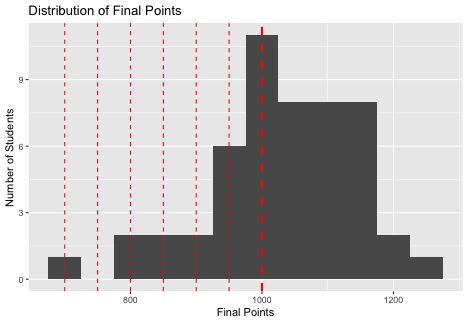
\includegraphics{figures/points-distribution-1.png}

There were 31 students who earned an A. Among those who earned an A,
their average points were 1096.419. This means that the A students
averaged \textbf{96.419} points too many than they needed. This is
relative to the overall mean of 1028.255

\subsection{Assessment Choices}\label{assessment-choices}

\subsubsection{Aggregated}\label{aggregated}

\begin{Shaded}
\begin{Highlighting}[]
\NormalTok{assignment.summary.data <-}
\StringTok{  }\NormalTok{assessment.dataset %>%}
\StringTok{  }\KeywordTok{group_by}\NormalTok{(Assignment) %>%}
\StringTok{  }\KeywordTok{summarize}\NormalTok{(}\DataTypeTok{Mean.Points =} \KeywordTok{mean}\NormalTok{(Points)) %>%}
\StringTok{  }\KeywordTok{arrange}\NormalTok{(-Mean.Points)}

\NormalTok{positions <-}\StringTok{ }\KeywordTok{as.character}\NormalTok{(assignment.summary.data$Assignment)}

\KeywordTok{library}\NormalTok{(forcats)}

\NormalTok{assignment.summary.data$Assignment <-}\StringTok{ }\KeywordTok{fct_relevel}\NormalTok{(assignment.summary.data$Assignment, positions)}

\NormalTok{p <-}\StringTok{ }\KeywordTok{ggplot}\NormalTok{(assignment.summary.data, }\KeywordTok{aes}\NormalTok{(}\DataTypeTok{y=}\NormalTok{Mean.Points, }\DataTypeTok{x=}\NormalTok{Assignment))}
\NormalTok{p +}\StringTok{ }\KeywordTok{geom_bar}\NormalTok{(}\DataTypeTok{stat=}\StringTok{'identity'}\NormalTok{, }\KeywordTok{aes}\NormalTok{(}\DataTypeTok{fill=}\NormalTok{Assignment)) +}\StringTok{ }\KeywordTok{scale_x_discrete}\NormalTok{(}\DataTypeTok{limits =} \NormalTok{positions) +}\StringTok{   }
\StringTok{  }\KeywordTok{labs}\NormalTok{(}\DataTypeTok{title=}\StringTok{"Aggregate Assignment Breakdown"}\NormalTok{,  }\DataTypeTok{y =} \StringTok{"Average Points"}\NormalTok{) +}
\StringTok{  }\KeywordTok{theme}\NormalTok{(}\DataTypeTok{axis.title.x=}\KeywordTok{element_blank}\NormalTok{(),}
        \DataTypeTok{axis.text.x=}\KeywordTok{element_blank}\NormalTok{(),}
        \DataTypeTok{axis.ticks.x=}\KeywordTok{element_blank}\NormalTok{())}
\end{Highlighting}
\end{Shaded}

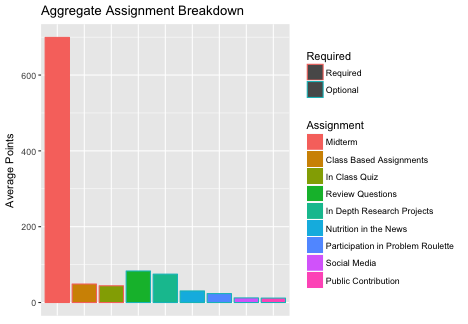
\includegraphics{figures/points-from-assessments-summary-1.png}

\begin{Shaded}
\begin{Highlighting}[]
\NormalTok{p <-}\StringTok{ }\KeywordTok{ggplot}\NormalTok{(}\KeywordTok{filter}\NormalTok{(assignment.summary.data, Assignment !=}\StringTok{ 'Midterm'}\NormalTok{), }\KeywordTok{aes}\NormalTok{(}\DataTypeTok{y=}\NormalTok{Mean.Points, }\DataTypeTok{x=}\NormalTok{Assignment))}
\NormalTok{p +}\StringTok{ }\KeywordTok{geom_bar}\NormalTok{(}\DataTypeTok{stat=}\StringTok{'identity'}\NormalTok{, }\KeywordTok{aes}\NormalTok{(}\DataTypeTok{fill=}\NormalTok{Assignment)) +}\StringTok{ }\KeywordTok{scale_x_discrete}\NormalTok{(}\DataTypeTok{limits =} \NormalTok{positions) +}\StringTok{   }
\StringTok{  }\KeywordTok{labs}\NormalTok{(}\DataTypeTok{title=}\StringTok{"Aggregate Assignment Breakdown - Excluding Midterm"}\NormalTok{, }\DataTypeTok{y =} \StringTok{"Average Points"}\NormalTok{) +}
\StringTok{  }\KeywordTok{theme}\NormalTok{(}\DataTypeTok{axis.title.x=}\KeywordTok{element_blank}\NormalTok{(),}
        \DataTypeTok{axis.text.x=}\KeywordTok{element_blank}\NormalTok{(),}
        \DataTypeTok{axis.ticks.x=}\KeywordTok{element_blank}\NormalTok{())}
\end{Highlighting}
\end{Shaded}

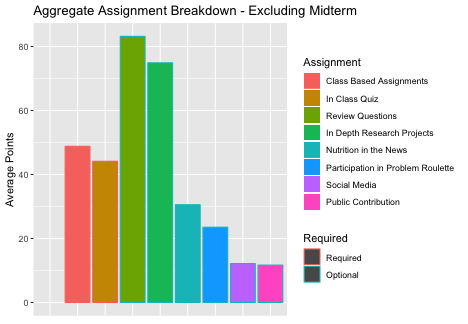
\includegraphics{figures/points-from-assessments-summary-2.png}

\subsubsection{Student Level}\label{student-level}

\begin{Shaded}
\begin{Highlighting}[]
\NormalTok{assessment.dataset$Username <-}\StringTok{ }\KeywordTok{fct_relevel}\NormalTok{(assessment.dataset$Username, summary.dataset$Username)  }
\NormalTok{assessment.dataset$Assignment <-}\StringTok{ }\KeywordTok{fct_relevel}\NormalTok{(assessment.dataset$Assignment, positions)}

\NormalTok{p <-}\StringTok{ }\KeywordTok{ggplot}\NormalTok{(assessment.dataset, }\KeywordTok{aes}\NormalTok{(}\DataTypeTok{y=}\NormalTok{Points,}\DataTypeTok{x=}\NormalTok{Username))}

\NormalTok{p +}\StringTok{ }\KeywordTok{geom_bar}\NormalTok{(}\DataTypeTok{stat=}\StringTok{'identity'}\NormalTok{, }\KeywordTok{aes}\NormalTok{(}\DataTypeTok{fill=}\NormalTok{Assignment)) +}
\StringTok{  }\KeywordTok{labs}\NormalTok{(}\DataTypeTok{title=}\StringTok{"Student Level Assignment Breakdown"}\NormalTok{) +}
\StringTok{  }\KeywordTok{theme}\NormalTok{(}\DataTypeTok{axis.title.x=}\KeywordTok{element_blank}\NormalTok{(),}
        \DataTypeTok{axis.text.x=}\KeywordTok{element_blank}\NormalTok{(),}
        \DataTypeTok{axis.ticks.x=}\KeywordTok{element_blank}\NormalTok{()) +}
\StringTok{    }\KeywordTok{geom_hline}\NormalTok{(}\KeywordTok{aes}\NormalTok{(}\DataTypeTok{yintercept=}\DecValTok{1000}\NormalTok{), }\DataTypeTok{color=}\StringTok{"black"}\NormalTok{, }\DataTypeTok{linetype=}\StringTok{"dashed"}\NormalTok{, }\DataTypeTok{size=}\FloatTok{0.5}\NormalTok{) }
\end{Highlighting}
\end{Shaded}

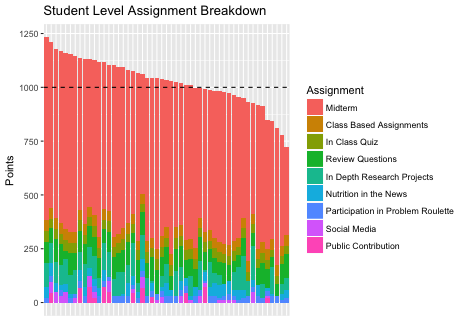
\includegraphics{figures/points-from-assessments-individual-1.png}


\end{document}
